\section{Systematic uncertainties}
\label{sec:syst}

\begin{figure} [!h]
  \begin{center}
    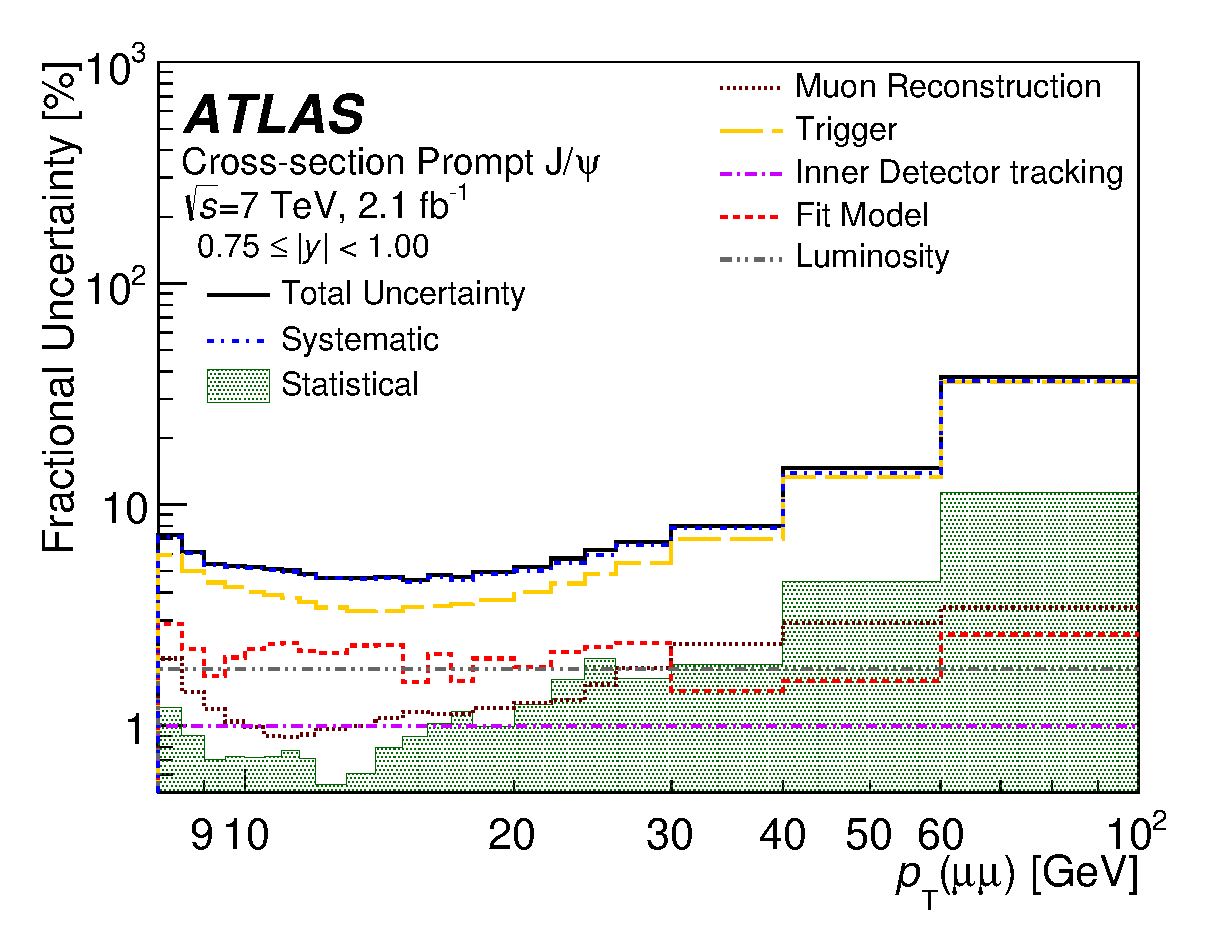
\includegraphics[width=0.49\textwidth]{hs_all_rap_0p75_1p00_jpsiP.eps}
    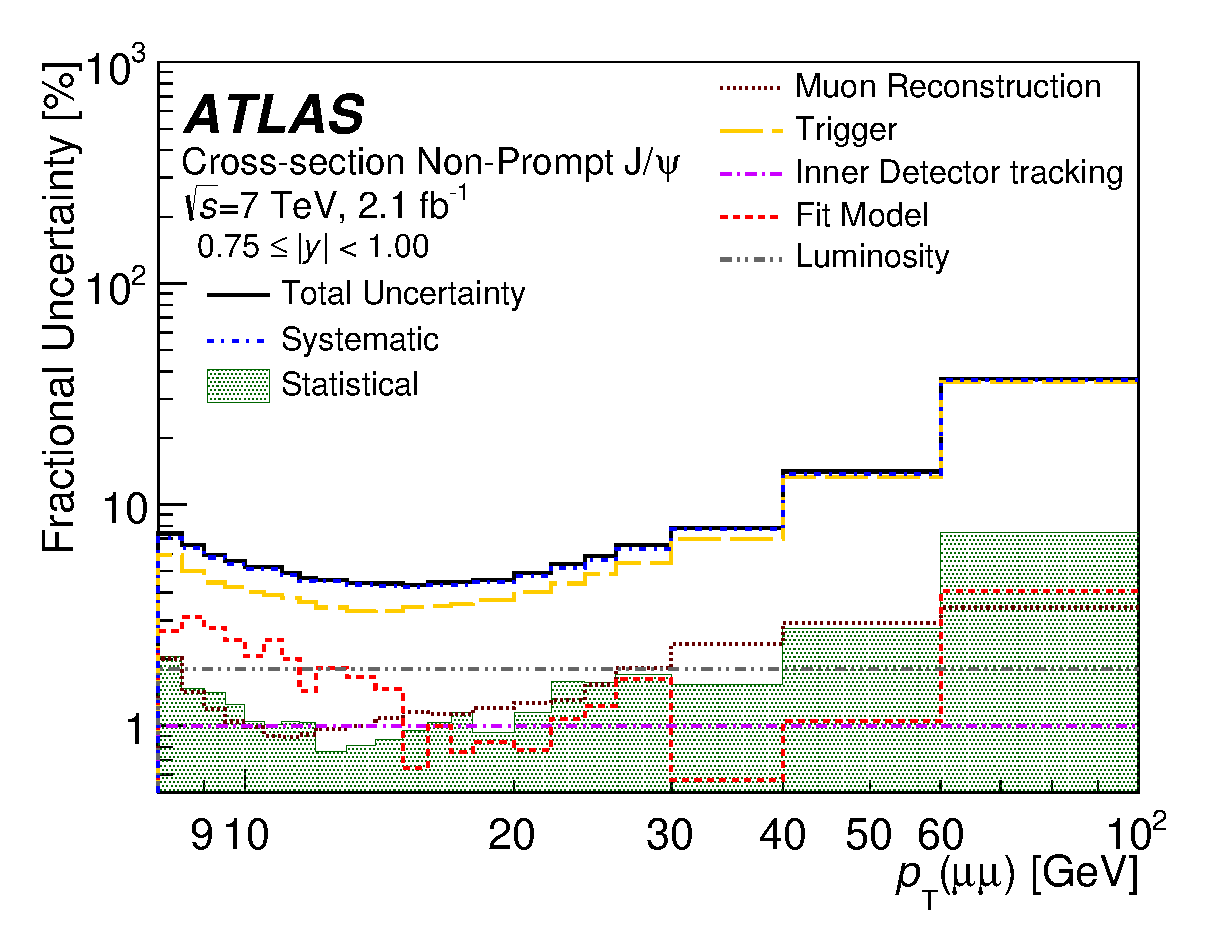
\includegraphics[width=0.49\textwidth]{hs_all_rap_0p75_1p00_jpsiNP.eps}\\
    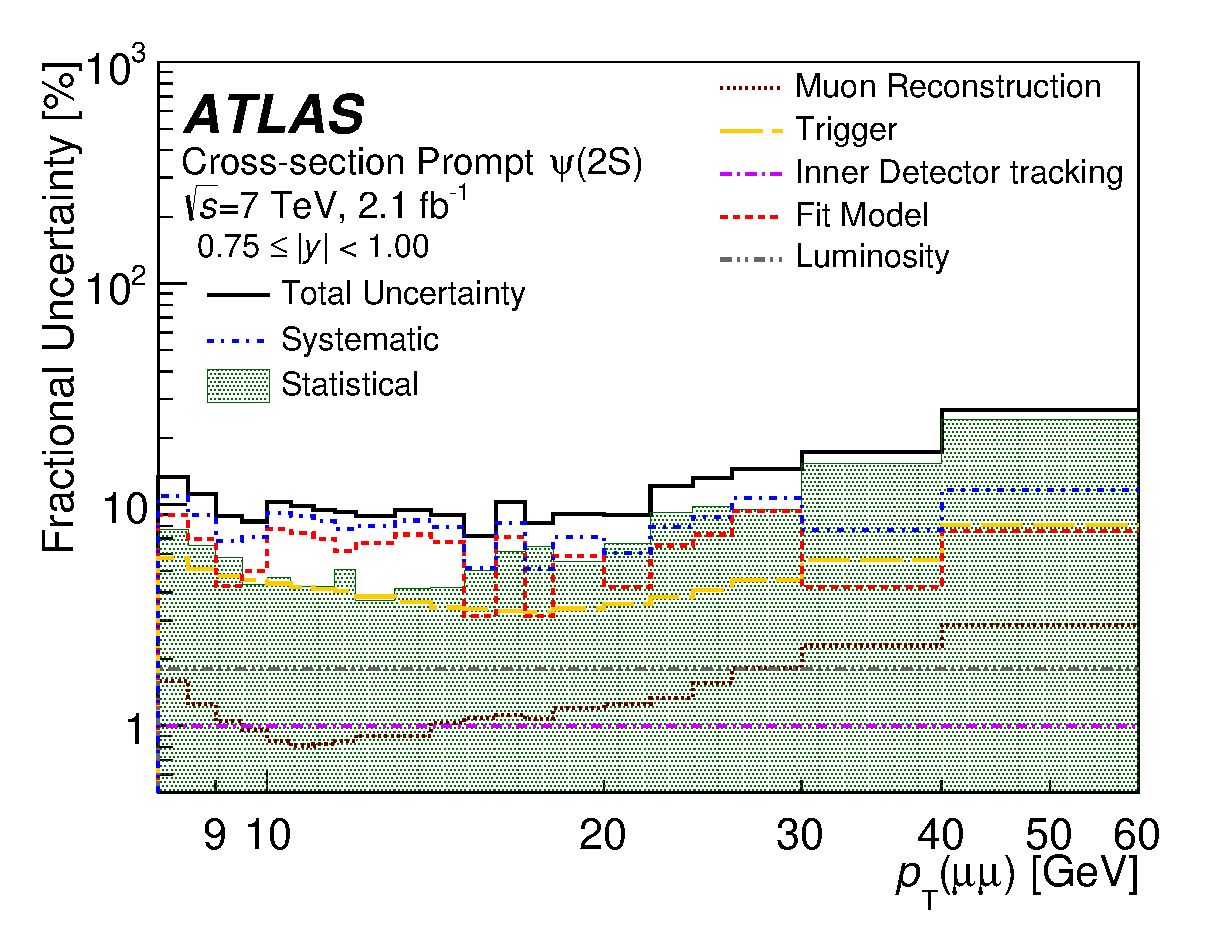
\includegraphics[width=0.49\textwidth]{hs_all_rap_0p75_1p00_psi2sP.eps}
    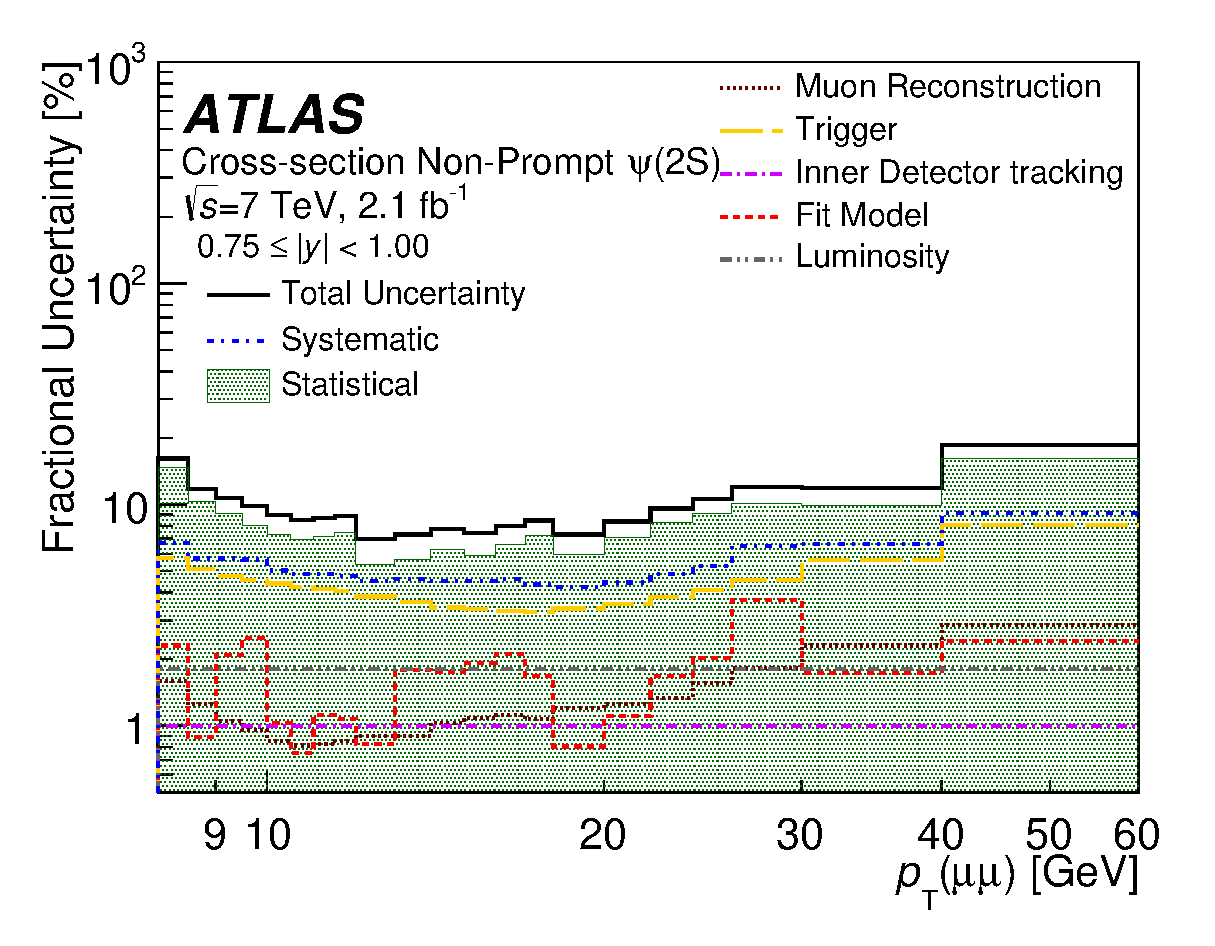
\includegraphics[width=0.49\textwidth]{hs_all_rap_0p75_1p00_psi2sNP.eps}    
    \caption{Statistical and systematic contributions to the fractional uncertainty on the prompt (left column) and non-prompt (right column)
    $\jpsi$ (top row) and $\psiprime$ (bottom row) cross-sections for 7 \TeV, 
    shown for the region $0.75<|y|<1.00$.}
    \label{fig:fracsyst_xs}
  \end{center}
\end{figure}

\begin{figure} [!h]
  \begin{center}
    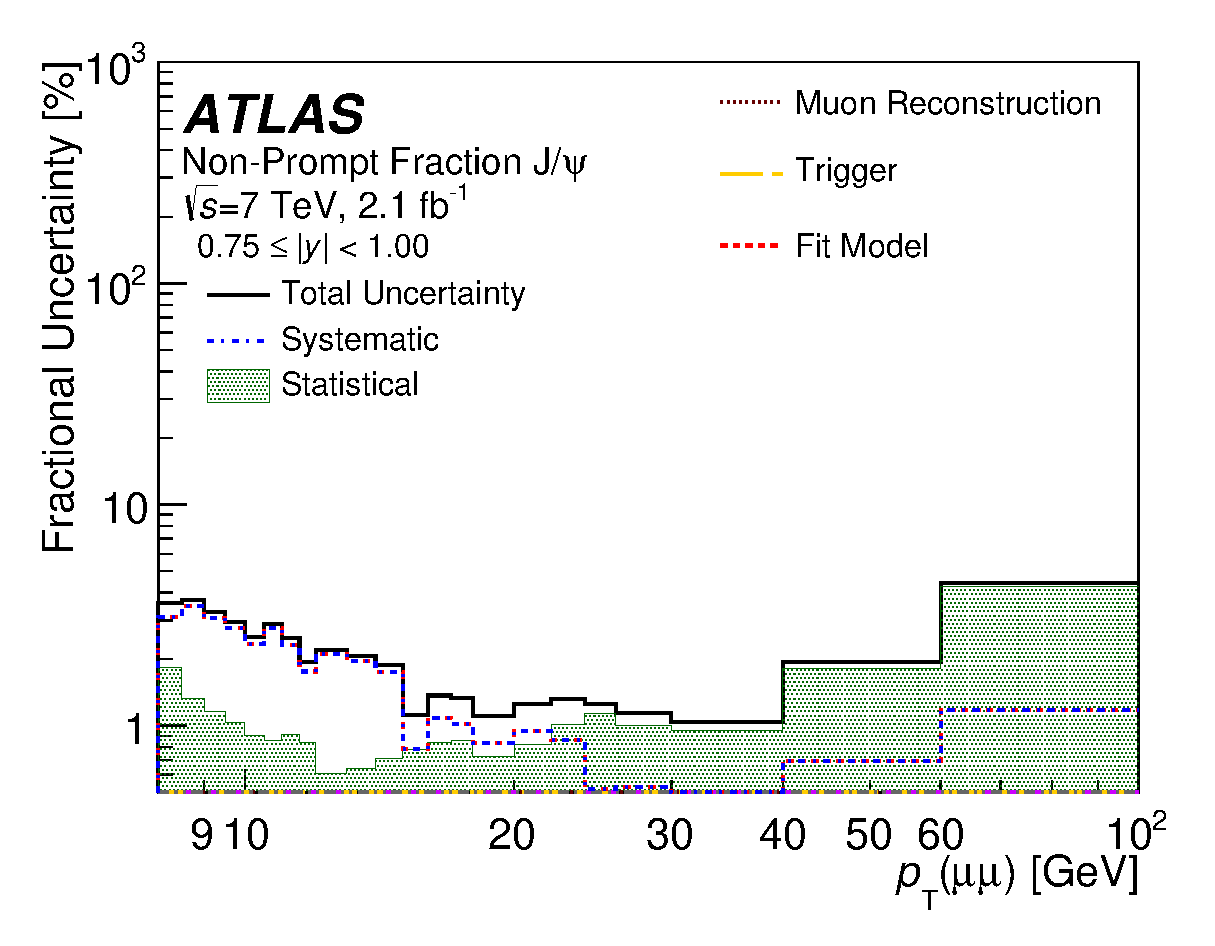
\includegraphics[width=0.49\textwidth]{hs_all_rap_0p75_1p00_fNPjpsi.eps}
    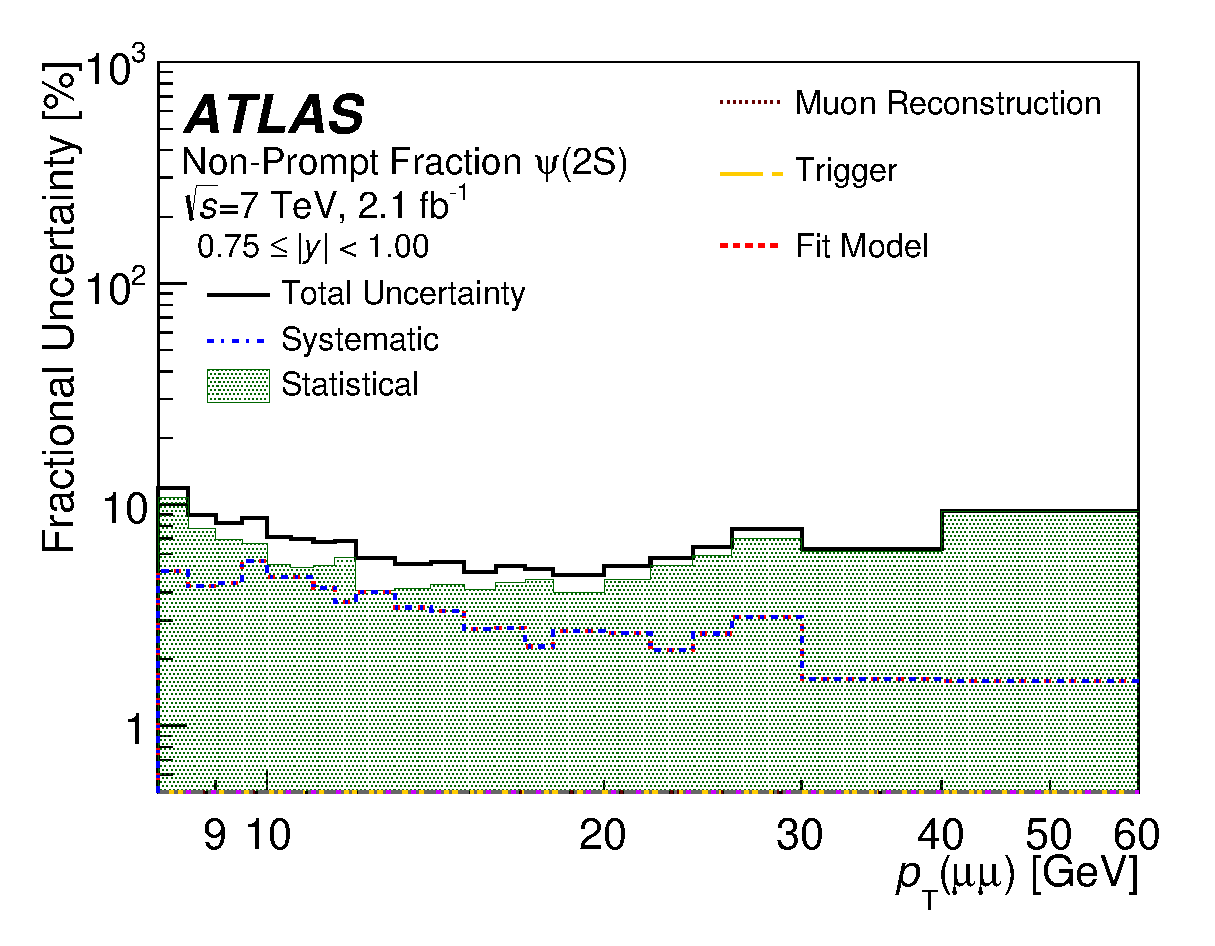
\includegraphics[width=0.49\textwidth]{hs_all_rap_0p75_1p00_fNPpsi2s.eps}\\
    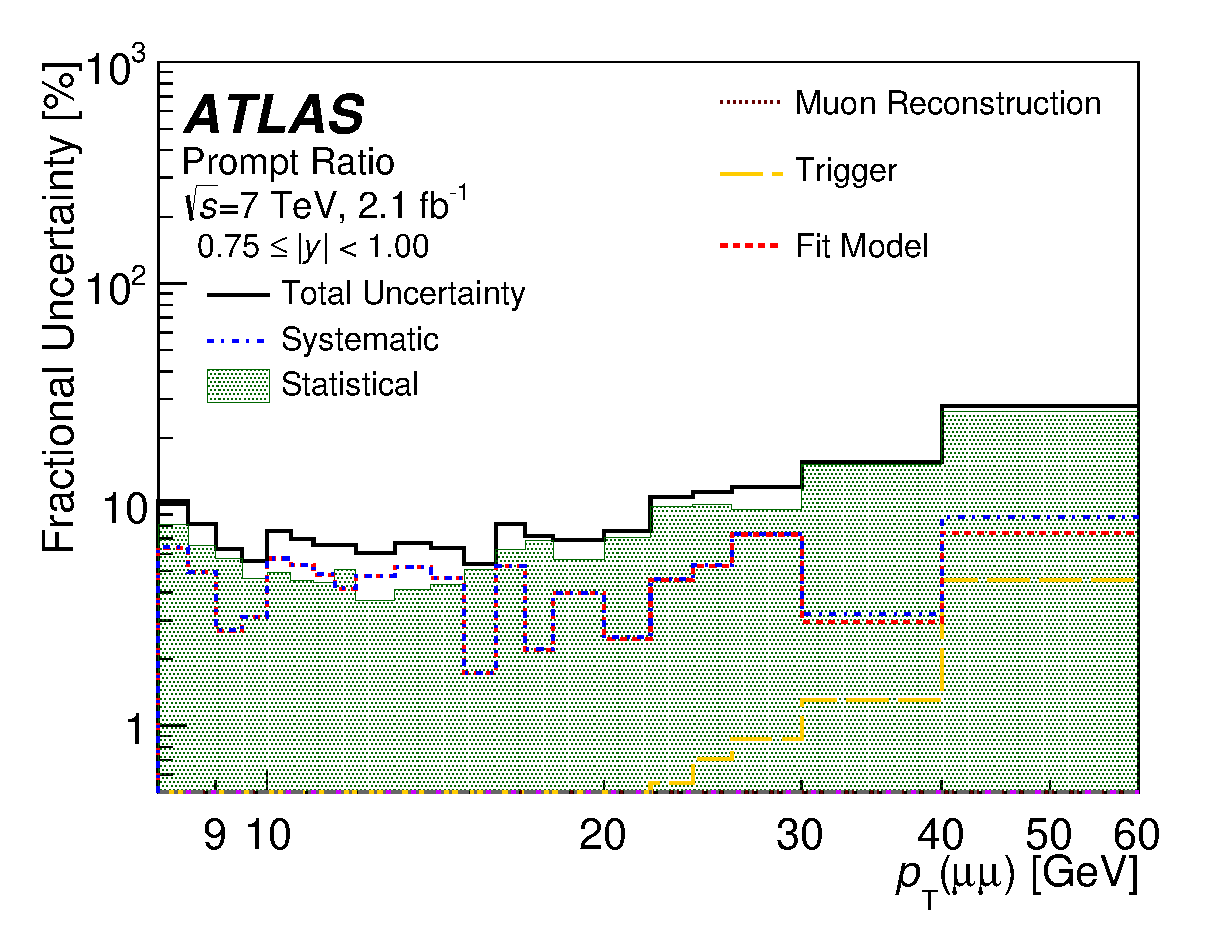
\includegraphics[width=0.49\textwidth]{hs_all_rap_0p75_1p00_ratioP.eps}
    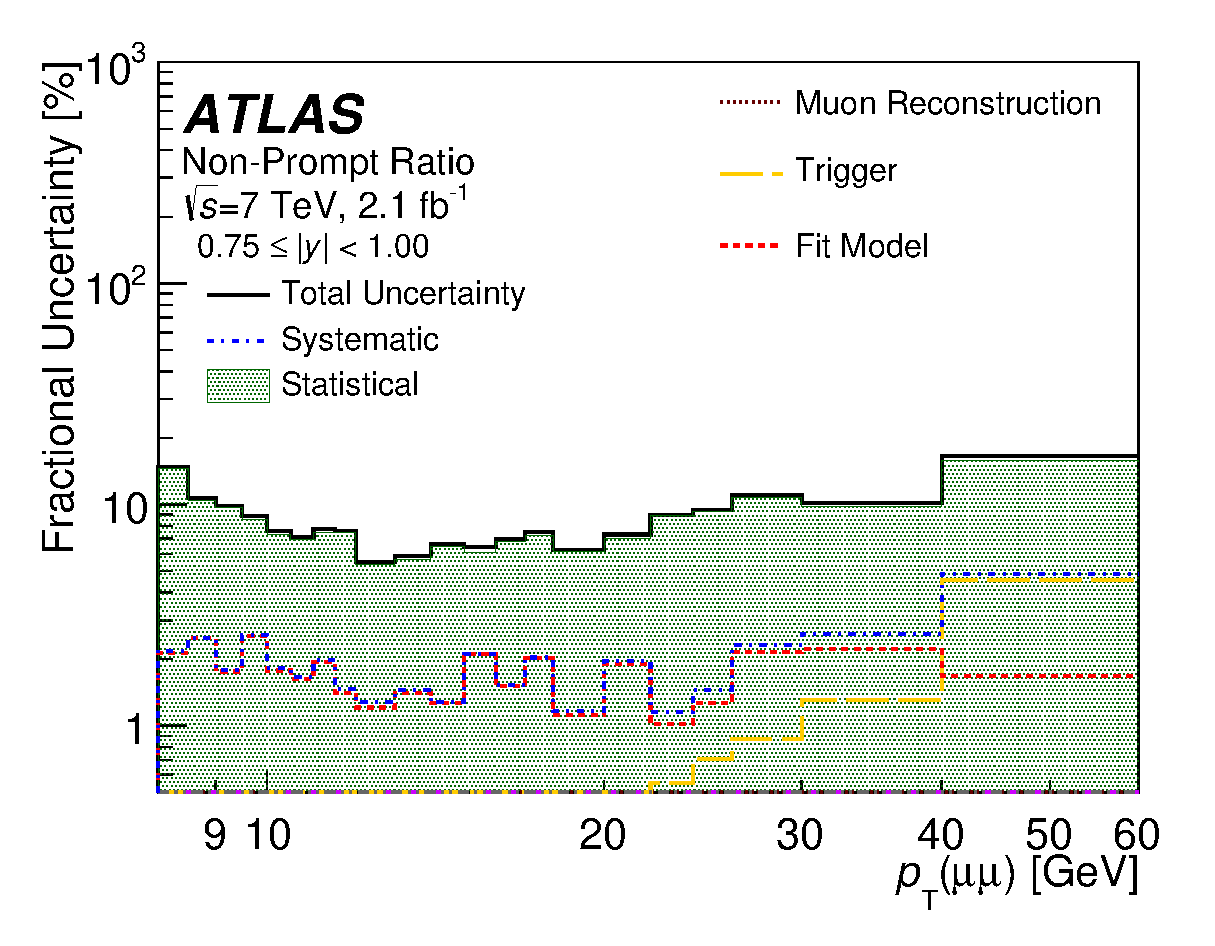
\includegraphics[width=0.49\textwidth]{hs_all_rap_0p75_1p00_ratioNP.eps} 
    \caption{Breakdown of the contributions to the fractional uncertainty on the non-prompt fractions for $\jpsi$ (top left) and $\psiprime$ (top right), 
    and the prompt (bottom left) and non-prompt (bottom right) ratios for 7 \TeV, 
    shown for the region $0.75<|y|<1.00$.}
    \label{fig:fracsyst_ratio}
  \end{center}
\end{figure}


The sources of systematic uncertainty evaluated for these measurements, along with the minimum, maximum and median values, are listed in Table~\ref{table:systlist}.
The largest contributions, which originate from the trigger and fit model uncertainties, are typically for the 
high $\pt$ intervals and are due to the limited statistics of the efficiency maps (for the trigger), and the data sample (for the fit model).

The impact of these uncertainties on the production cross-section measurements, 
as well as on their ratios for 7 \TeV\ data, is shown for a representative interval in
Figures~\ref{fig:fracsyst_xs} and~\ref{fig:fracsyst_ratio}, respectively.
The impact is very similar at 8 \TeV.


\begin{table}[h!]
 \caption{Summary of the minimum and maximum contributions along with the median of the systematic uncertainties as percentages. Values are quoted for 7 and 8 \TeV\ data.}
 \centering
    \begin{tabular}{l || c c c | c c c  }
    \hline 
     & \multicolumn{3}{c|}{7 \TeV\ [\%]} & \multicolumn{3}{c}{8 \TeV\ [\%]} \\
    \hline 
    Source of systematic uncertainty                   & Min & Median & Max & Min & Median & Max \\
    Luminosity                         & 1.8 & 1.8 & 1.8    & 2.8 & 2.8 & 2.8 \\
    Muon reconstruction efficiency     & 0.7 & 1.2 & 4.7    & 0.3 & 0.7 & 6.0 \\
    Muon trigger efficiency            & 3.2 & 4.7 & 35.9   & 2.9 & 7.0 & 23.4 \\
    Inner detector tracking efficiency & 1.0 & 1.0 & 1.0    & 1.0 & 1.0 & 1.0 \\
    Fit model parameterizations        & 0.5 & 2.2 & 22.6   & 0.26 & 1.07 & 24.9 \\
    Bin migrations                     & 0.01 & 0.1 & 1.4   & 0.01 & 0.3 & 1.5 \\ \hline
    Total                              & 4.2 & 6.5  & 36.3  & 4.4 & 8.1 & 27.9 \\
    \hline  
      \hline
    \end{tabular}
\label{table:systlist}
\end{table}


\setdescription{font=\normalfont\itshape}

\begin{description}[style=unboxed,leftmargin=0cm]
\item[Luminosity] \hfill \\
The uncertainty on the integrated luminosity is $1.8\%$ ($2.8\%$) for the 7~\TeV\ (8~\TeV) data-taking period.  
The methodology used to determine these uncertainties is described in Ref.~\cite{Aad:2013ucp}.
The luminosity uncertainty is only applied to the \jpsi\ and \psiprime\ cross-section results.


\item[Muon reconstruction and trigger efficiencies] \hfill \\
To determine the systematic uncertainty on the muon reconstruction and trigger efficiency maps, each of the maps is reproduced in 100 pseudo-experiments.
The dominant uncertainty in each bin is statistical and hence any bin-to-bin correlations are neglected.
For each pseudo-experiment a new map is created by varying independently each bin content according to a Gaussian distribution about its estimated value, 
determined from the original map.
In each pseudo-experiment, the total weight is recalculated for each dimuon $\pt$ and $|y|$ interval of the analysis.
The RMS of the total weight pseudo-experiment distributions for each efficiency type is used as the systematic uncertainty,
where any correlation effects between the muon and trigger efficiencies can be neglected.


The ID tracking efficiency is in excess of $99.5\%$ \cite{Aad2012dlq}, and
an uncertainty of 1\% is applied to account for the ID dimuon reconstruction inefficiency (0.5\% per muon, added coherently). This
uncertainty is applied to the differential cross-sections and is assumed to cancel in the ratio of non-prompt to inclusive production for \jpsi\ and 
\psiprime\ and in the ratios of \psiprime\ to \jpsi\ production.

For the trigger efficiency  $\epsilon_\mathrm{trig}$, there is an additional correction that accounts for correlations between the two trigger muons. This 
correction is varied by its uncertainty, and the shift in the resultant total weight relative to its central value is added in quadrature to the uncertainty from the map.
The choice of triggers is known \cite{Aad:2014cqa} to introduce a small lifetime-dependent efficiency loss but it is determined to have a negligible effect on 
the prompt and non-prompt yields and no correction is applied in this analysis.

  \item[Fit model uncertainty] \hfill \\
The uncertainty due to the fit procedure is determined by varying one component at a
time in the fit model described in Section \ref{sec:method:fit}, creating a set of new fit models. For each new
fit model, all measured quantities are recalculated, and in each $\pt$ and $|y|$ interval the spread of
variations around the central fit model is used as its systematic uncertainty.
The following variations to the central model fit are evaluated: 

\begin{itemize}

  \item  signal mass model --- using double Gaussian models in place of the Crystal Ball plus Gaussian model;  variation of the
 $\alpha$ and $n$ parameters of the $B$ model, which are originally fixed;

    \item  signal pseudo-proper decay time model --- a double exponential function is used to describe the pseudo-proper decay time distribution for the 
    $\apsi$ non-prompt signal;

  \item  background mass models --- variations of the mass model using exponentials functions, or quadratic Chebyshev polynomials to describe the components of prompt,
 non-prompt and double-sided background terms;

  \item  background pseudo-proper decay time model --- a single exponential function was considered for the non-prompt component;

  \item  pseudo-proper decay time resolution model --- using a single Gaussian function in place of the double Gaussian function to model the lifetime resolution
 (also prompt lifetime model); and variation of the mixing terms for the two Gaussian components of this term.

\end{itemize}

  \item[Bin migrations] \hfill \\
As the corrections to the results due to bin migration effects are factors close to unity in all regions, the difference between the correction factor and unity is applied as the uncertainty. 

\end{description}

